\documentclass[a4paper,12pt]{article}

\newcommand{\ind}[1]{\ensuremath{_{\rm{#1}}}}
\newcommand{\expo}[1]{\ensuremath{^{\rm{#1}}}}


\usepackage{amsmath}
\usepackage{amssymb}
\usepackage{graphicx}

\setlength\parindent{0in}
\oddsidemargin 0.0in
\evensidemargin 1.0in
\textwidth 6.0in
\textheight 9.0in
\headheight 0.0in
\topmargin 0.0in

% Title Page
\title{CHEASE/NEOART Interface}
\author{Y. Camenen}
\date{November 11, 2009}

\begin{document}
\maketitle

%\begin{abstract}
%
%\end{abstract}

Documents the addition of a small module in CHEASE to compute the quantities required for NEOART and of another module in NEOART to read the CHEASE outputs.


%*********************************************************************
\section{CHEASE modification}
%*********************************************************************

A new subroutine \texttt{neoart.f90} (based on \texttt{hamada.f90}) is added to output the quantities required for NEOART. All the quantities in the output file are in SI units. The names of
the various quantities in the output file are chosen to be the same than the ones in the subroutine \texttt{geom.f} of NEOART.
New quantities are calculated in \texttt{surface.f90}
\subsection{Conventions}


\subsection{Outputs}
\textbf{Scalars}\\
NPSI: number of points for the radial grid\\
R0EXP: reference major radius used in CHEASE, generally taken to be close to the magnetic axis radius for faster convergence (but the actual position is not necessarily known beforehand)\\
B0EXP: reference magnetic field in CHEASE defined as the magnetic field at R0EXP\\
Raxis: magnetic axis radius as calculated by CHEASE
\vspace{0.5cm}

\textbf{Grid}\\
PSI: $\Psi$, the poloidal flux, zero at the magnetic axis, increasing towards the edge
\vspace{0.5cm}

\textbf{1D arrays}\\
Rgeom: major radius of the flux surface centre, defined as $(R\ind{max}+R\ind{min})/2$\\
amin: minor radius of the flux surface, defined as $(R\ind{max}-R\ind{min})/2$\\
damindpsi: $\partial \mathrm{amin}/\partial \Psi$\\
bmax: maximum of the magnetic field strength on the flux surface\\
bmin: minimum of the magnetic field strength on the flux surface\\
q: safety factor\\
dqdpsi: $\partial q /\partial \Psi$\\
p: plasma pressure\\
dpdpsi: $\partial p /\partial \Psi$\\
f: $F=RB\ind{t} = R^2|\mathbf{B}\cdot\nabla\phi|$ (always positive by convention)\\
dfdpsi: $\partial F /\partial \Psi$\\
bav: flux surface average of the magnetic field strength $< B >$\\
b2av: $< B^2 >$\\
bi2av: $< 1/B^2 >$\\
r2av: $< R^2 >$\\
ri2av: $< 1/R^2 >$\\
gclass: $< R^2B\ind{p}^2/B^2 > = <R^2>-F^2<1/B^2>$\\
bgradp: $\mathbf{b}\cdot\nabla \Theta$, as defined in Houlberg's paper PoP \textbf{4} 3230 (1997)\\
fm1 to fm6: $F\ind{M}$ coefficients for the Pfirsch-Schlutter contribution to the viscosity integral, equation B9 in Houlberg PoP \textbf{4} 3230 (1997)

\subsection{Checks}
The quantities calculated in CHEASE for an equilibrium with circular flux surfaces are compared to the analytical expressions (extracted from the \texttt{geom.f} module of NEOART). The
reference radius is $R\ind{N}=R\ind{axis}$, the reference magnetic field is $B\ind{N}=B(R\ind{geom})$ and the inverse aspect ratio $\epsilon =\frac{R\ind{max}-R\ind{min}}{2R\ind{N}}$. The following
expressions are used for the comparison:
$$\textrm{BAV}=<B>=B\ind{N}$$
$$\textrm{B2AV}=<B^2>=\frac{B\ind{N}^2}{\sqrt{1-\epsilon^2}}$$
$$\textrm{BI2AV}=<1/B^2>=\frac{1+1.5\epsilon^2}{B\ind{N}^2}$$
$$\textrm{RBT}=F=R\ind{N}B\ind{N}\frac{\sqrt{1-\epsilon^2}}{\sqrt{1+\epsilon^2(1/q^2-1)}}$$
$$\textrm{BGRADP}=\mathbf{b}\cdot\nabla \Theta=\frac{1}{R\ind{N}\sqrt{\epsilon^2+q^2(1-\epsilon^2)}}$$
$$\textrm{DPSIDR}=\frac{\partial\Psi}{\partial\rho}=\frac{R\ind{N}B\ind{N}}{\sqrt{1+q^2(1/\epsilon^2-1)}}$$
$$\textrm{RNQ}=R\ind{N}q$$
$$\textrm{FC}=(1-\epsilon)\sum_{i=0}^5 a_i \epsilon^{i/2}$$
with the coefficients taken to be $a_0=1$, $a_1=-1.46655$, $a_2=1.0241$, $a_3=-1.20107$, $a_4=1.356234$, $a_5=-0.662881$
$$\textrm{GCLASS}=\frac{\epsilon^2 R\ind{N}^2(1+1.5\epsilon^2)}{q^2+\epsilon^2(1-q^2)}$$
$$\textrm{FM}(i)=2i(\mathbf{b}\cdot\nabla\Theta)^2\left[\frac{-1+\sqrt{1-\epsilon^2}}{\epsilon}\right]^{2i}$$
$$\textrm{R2I}=<1/R^2>=\frac{1}{R\ind{N}^2\sqrt{1-\epsilon^2}}$$
\begin{figure}[!htb]
        \begin{center}
        \includegraphics[width=0.45\columnwidth]{/storage/space1/phsgbe/codes/neoart/test_geom/bav.eps}%
        \includegraphics[width=0.45\columnwidth]{/storage/space1/phsgbe/codes/neoart/test_geom/b2av.eps}%
        \end{center}
\end{figure}
\begin{figure}[!htb]
        \begin{center}
        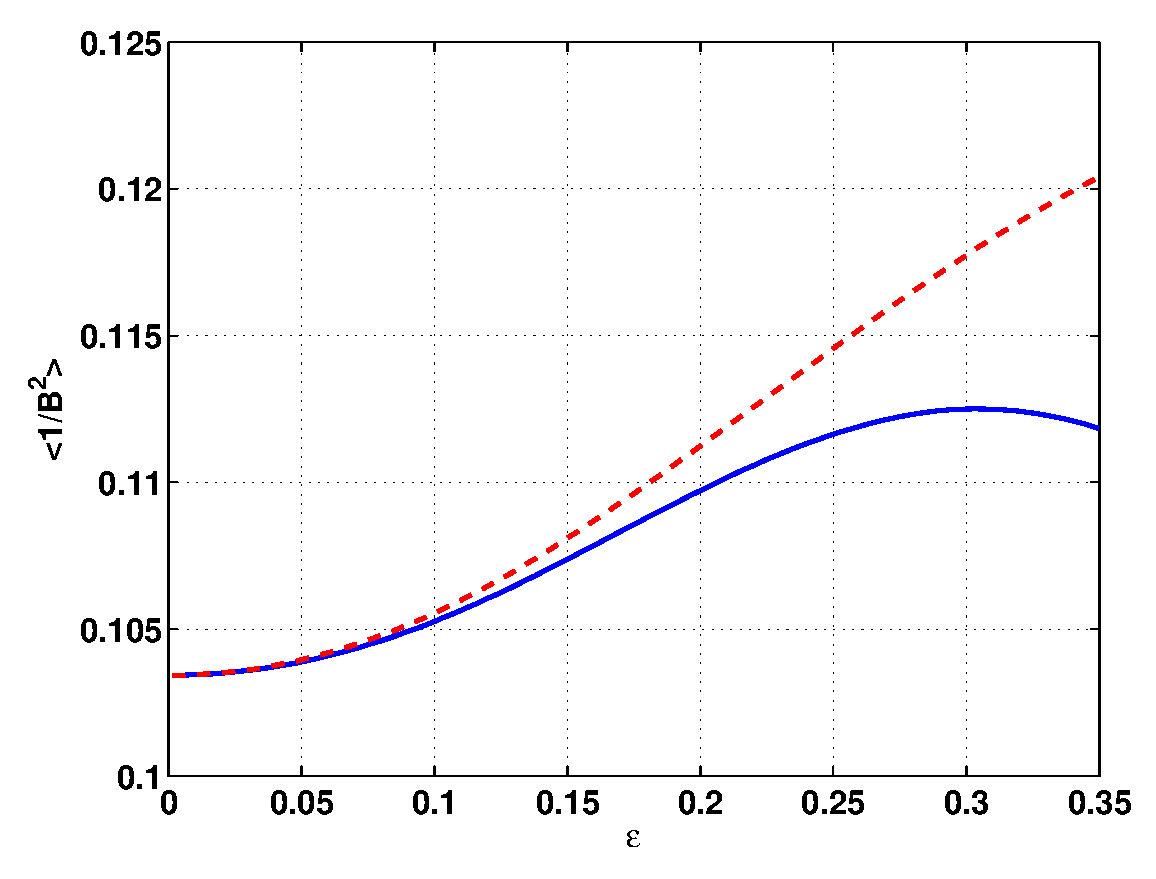
\includegraphics[width=0.45\columnwidth]{/storage/space1/phsgbe/codes/neoart/test_geom/bi2av.eps}%
        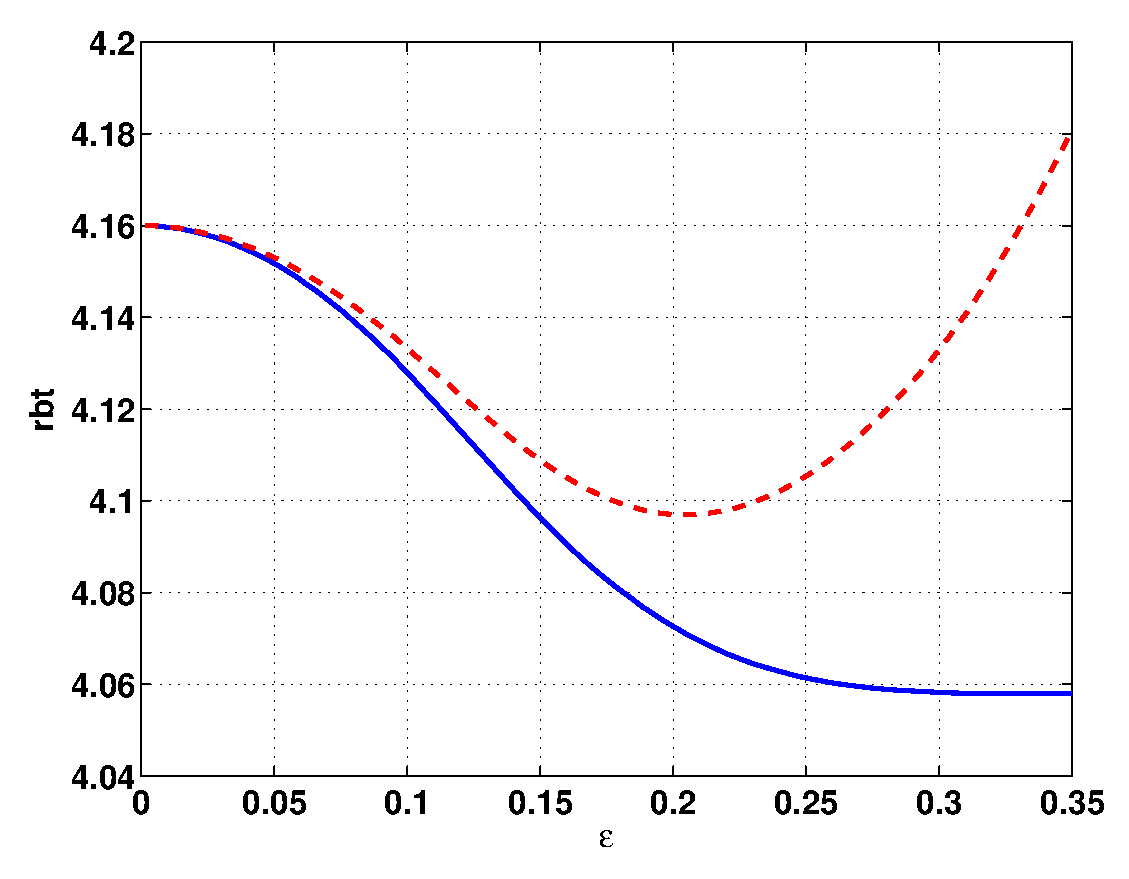
\includegraphics[width=0.45\columnwidth]{/storage/space1/phsgbe/codes/neoart/test_geom/rbt.eps}%
        \end{center}
\end{figure}
\begin{figure}[!htb]
        \begin{center}
        \includegraphics[width=0.45\columnwidth]{/storage/space1/phsgbe/codes/neoart/test_geom/bgradp.eps}%
        \includegraphics[width=0.45\columnwidth]{/storage/space1/phsgbe/codes/neoart/test_geom/dpsidr.eps}%
        \end{center}
\end{figure}
\begin{figure}[!htb]
        \begin{center}
        \includegraphics[width=0.45\columnwidth]{/storage/space1/phsgbe/codes/neoart/test_geom/rnq.eps}%
        \includegraphics[width=0.45\columnwidth]{/storage/space1/phsgbe/codes/neoart/test_geom/fc.eps}%
        \end{center}
\end{figure}
\begin{figure}[!htb]
        \begin{center}
        \includegraphics[width=0.45\columnwidth]{/storage/space1/phsgbe/codes/neoart/test_geom/gclass.eps}%
        \includegraphics[width=0.45\columnwidth]{/storage/space1/phsgbe/codes/neoart/test_geom/r2i.eps}%
        \end{center}
\end{figure}
\begin{figure}[!htb]
        \begin{center}
        \includegraphics[width=0.45\columnwidth]{/storage/space1/phsgbe/codes/neoart/test_geom/fm1.eps}%
        \includegraphics[width=0.45\columnwidth]{/storage/space1/phsgbe/codes/neoart/test_geom/fm2.eps}%
        \end{center}
\end{figure}
\begin{figure}[!htb]
        \begin{center}
        \includegraphics[width=0.45\columnwidth]{/storage/space1/phsgbe/codes/neoart/test_geom/fm3.eps}%
        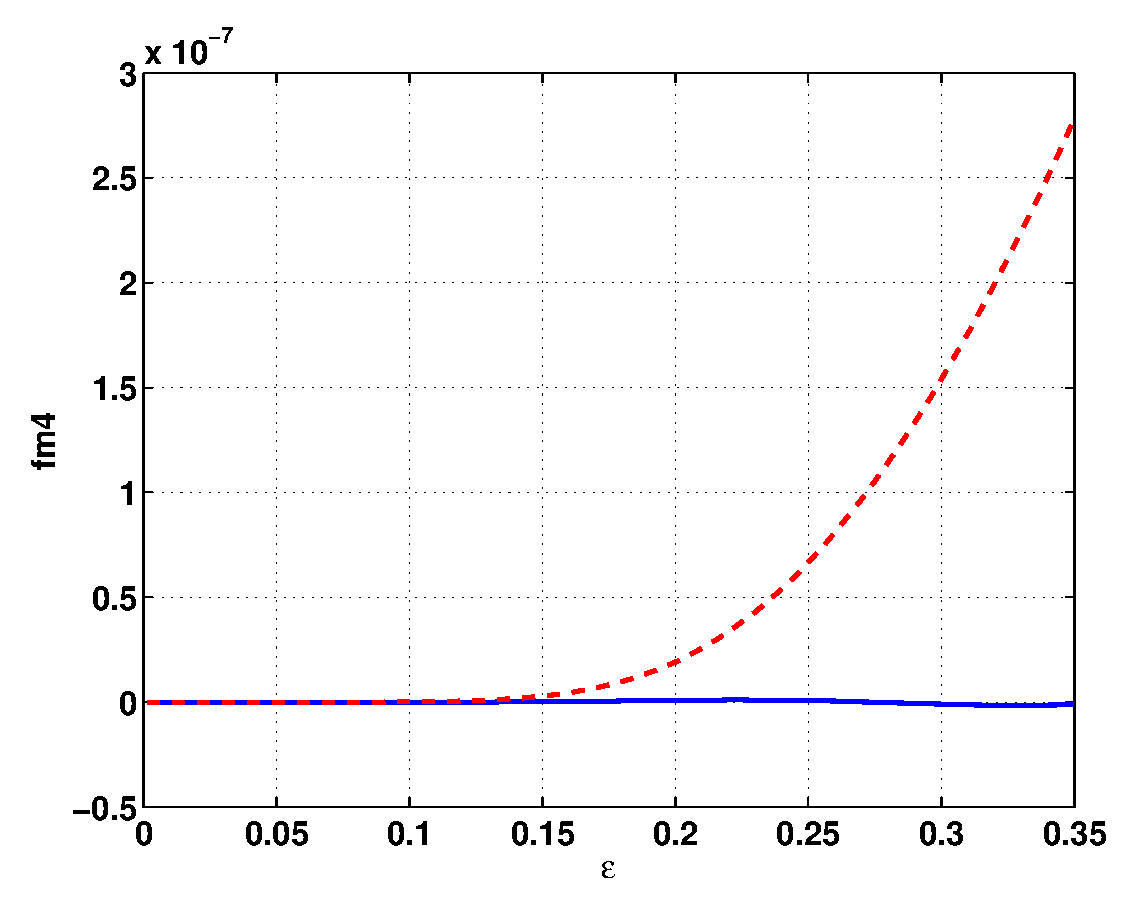
\includegraphics[width=0.45\columnwidth]{/storage/space1/phsgbe/codes/neoart/test_geom/fm4.eps}%
        \end{center}
\end{figure}
\begin{figure}[!htb]
        \begin{center}
        \includegraphics[width=0.45\columnwidth]{/storage/space1/phsgbe/codes/neoart/test_geom/fm5.eps}%
        \includegraphics[width=0.45\columnwidth]{/storage/space1/phsgbe/codes/neoart/test_geom/fm6.eps}%
        \end{center}
\end{figure}
\begin{figure}[!htb]
        \begin{center}
        \includegraphics[width=0.45\columnwidth]{/storage/space1/phsgbe/codes/neoart/test_geom/sumfm.eps}%
        \end{center}
\end{figure}

%*********************************************************************
\section{NEOART modification}
%*********************************************************************
The main change done in NEOART is the addition of a module \texttt{get\_geom\_ch.f} to load the data from the output file generated by CHEASE.
The full radial profiles are loaded and interpolated at the input radial value specified in NEOART.
The parameters related to the MHD equilibrium are read from the CHEASE output when NEOART is called with $\texttt{ISEL}=4$. The CHEASE output file has to be called \texttt{neoart\_geom.dat} and be
located in the directory where NEOART is run.
\end{document}
